\section{Question 11.2}

\subsection{Question}
Does your favorite web search engine use a bag of words representation?  How can you tell whether it does or doesn't?

\subsection{Answer}
My favorite search engine is Google.  I am fairly certain they do not limit their retrieval model to the simple bag-of-words model described by the text book.

As an example, there is a well known online meme, or trend, called "y u no guy".  It is an image macro used to bring attention to something and uses a popular practice for online forums of shortening words to their root sound corresponding to a letter, e.g. ``you'' becomes ``u''.  The target message is accompanied by a cartoon man with a face of frustration and rage.  See Figure \ref{fig:yuno} for the results of issuing the query ``y u no'' to Google's search engine.

\begin{figure}[H]
\centering
\label{fig:yuno}
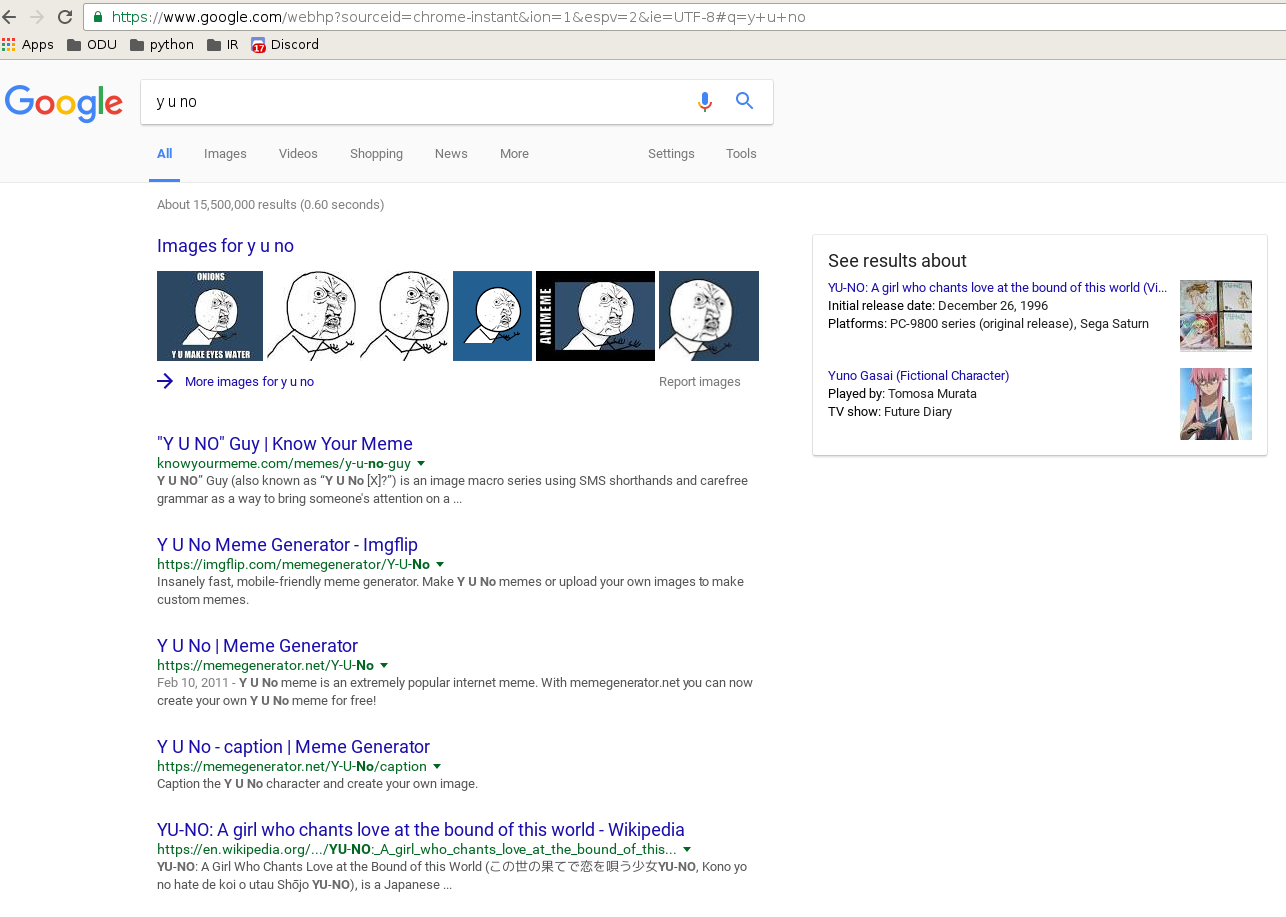
\includegraphics[scale=.25]{q11.2/yuno.png}
\caption{y u no guy}
\end{figure}

Google recognizes these three simple terms to be part of a phrase and retrieves results based on that phrase with a high degree of accuracy.

\clearpage

To show that Google's engine does not use the bag-of-words model, consider this similar search with the terms ``no u y''.

\begin{figure}[H]
\centering
\label{fig:nouy}
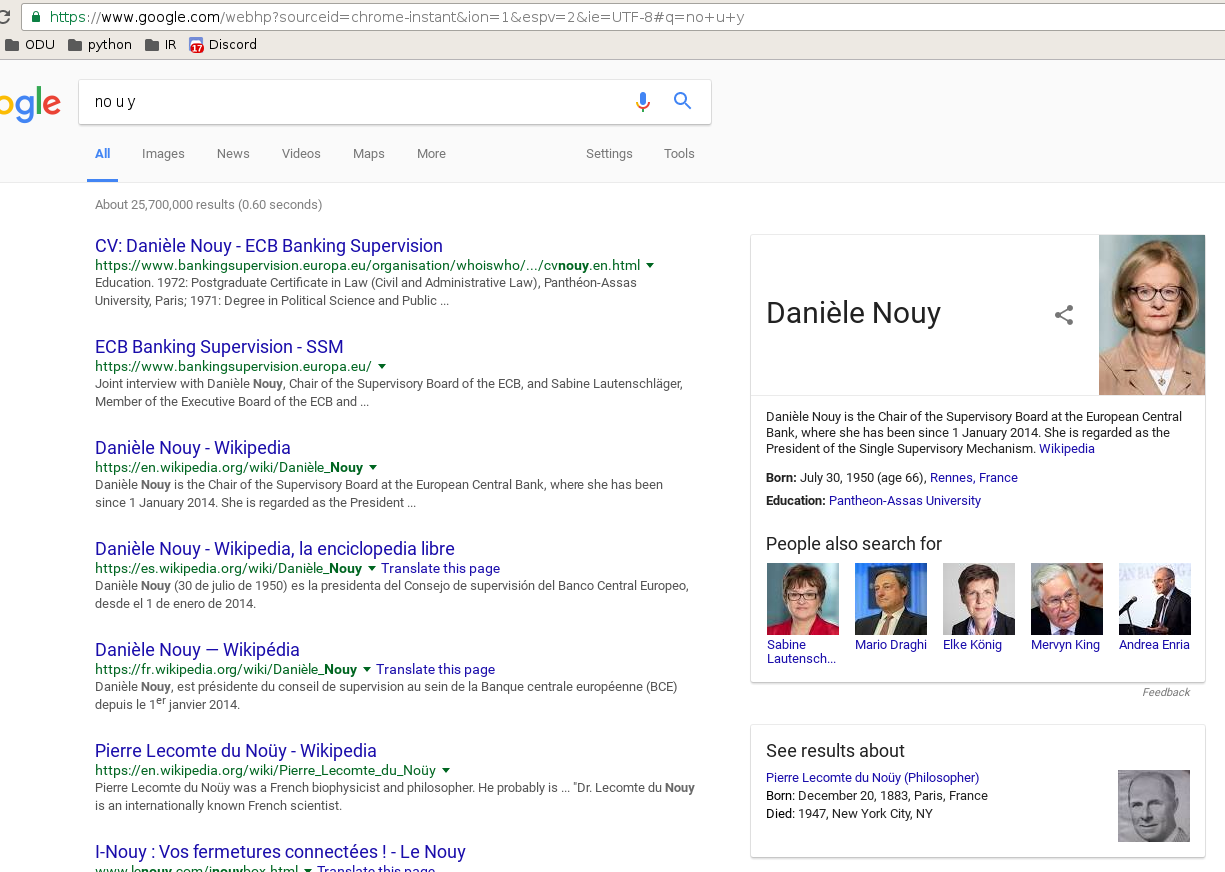
\includegraphics[scale=.25]{q11.2/nouy.png}
\caption{Daniele Nouy}
\end{figure}

With the same three terms in a different order, a completely different ranking is presented by the search engine.  The results for this search are not regarding y u no guy at all, they are dominated by pages about the Chair of the Supervisory Board at the European Central Bank, Daniele Nouy.  This shows that Google's engine accounts for query term ordering, which would not be present in a plain bag-of-words retrieval model.
